\documentclass[conference,a4paper]{IEEEtran}
\usepackage{fontspec}
\setmainfont{Liberation Serif}[SmallCapsFont={Latin Modern Roman Caps}]
\setsansfont{Liberation Sans}
\setmonofont{Liberation Mono}[Scale=MatchLowercase]
\usepackage{amsmath,amssymb}
\usepackage{graphicx}
\usepackage{booktabs,array}
\usepackage{cite}
\usepackage{url}
\usepackage{seqsplit}
\usepackage{balance}
\usepackage[hidelinks]{hyperref}
\newcommand{\splitsha}{\texttt{\seqsplit{55c87dabc5da1ef500560648ec40717cde381dec0410b3abab83cbdfceed1322}}}
\title{How Much Does Road-Damage Detection Degrade Across Acquisition Domains?\\A Scene-Aware Bidirectional Evaluation on RDD2022}
\author{\IEEEauthorblockN{Lê Thành Luân\IEEEauthorrefmark{1}, Phạm Bá Anh Tuấn\IEEEauthorrefmark{2}}\IEEEauthorblockA{University of Science and Technology -- The University of Danang, Da Nang, Vietnam\\\IEEEauthorrefmark{1}102250416@hv.dut.udn.vn; \IEEEauthorrefmark{2}102250421@hv.dut.udn.vn}}
\begin{document}
\maketitle

\begin{abstract}
Road-damage detectors may encounter acquisition conditions that differ substantially from their training imagery. This study measures bidirectional transfer between the China\_Drone and China\_MotorBike subsets of RDD2022 using a scene-reviewed partition and a fixed-target comparison: target-domain and other-domain training are evaluated on identical held-out target images. We analyze COCO-pretrained YOLOv8n, YOLO11n, and YOLO26n fine-tuned independently on each domain with three matched seeds and 150 epochs per run, yielding 18 training runs and 658 full-test images from a 4,378-image subset. The mean in-domain advantages in mAP@50:95 on Drone Test are $14.86\pm1.25$, $15.13\pm3.85$, and $16.91\pm0.80$ percentage points for YOLOv8n, YOLO11n, and YOLO26n, respectively. On MotorBike Test, the corresponding gaps are $41.24\pm1.04$, $42.94\pm0.52$, and $42.27\pm1.28$ points; uncertainties denote sample standard deviations across seeds. All 18 fixed-target seed comparisons favor target-domain training, and the same direction holds in an excluded-label sensitivity analysis. Class-level behavior is heterogeneous: D20 has a large gap on MotorBike Test, whereas sparse D40 annotations on Drone Test accompany negative mean class gaps. YOLO26n attains the highest mean in-domain mAP on both targets, but substantial cross-domain gaps remain. The results provide a descriptive three-variant replication; they do not isolate acquisition geometry from differences in training size, scene composition, or annotation distributions.
\end{abstract}

\begin{IEEEkeywords}
road damage detection, domain shift, RDD2022, YOLO, cross-domain evaluation, scene-aware splitting
\end{IEEEkeywords}

\section{Introduction}
Image-based road-damage detection can support pavement inspection by locating and classifying visible defects. Maeda \emph{et al.}\ introduced a smartphone-image benchmark and detection approach\cite{maeda2018road}; RDD2022 subsequently expanded the dataset to multiple countries and acquisition platforms\cite{arya2024rdd2022}. This diversity creates an operational question: how much accuracy is retained when training and deployment imagery come from different camera platforms? Strong performance on imagery resembling the training data does not answer that question.

Cross-domain comparisons require a clear reference. Subtracting a detector's score on Drone Test from its score on MotorBike Test changes the evaluation population as well as the acquisition domain. The difference therefore combines transfer behavior with differences in test-set composition and difficulty. We instead hold a target test set fixed and compare a detector trained on that target domain against a detector trained on the other domain. Repeating this comparison for both targets measures two target-trained advantages without treating different test populations as interchangeable.

We apply this design to the China\_Drone and China\_MotorBike subsets of RDD2022. A recorded scene-similarity audit informs the partition, and the same locked split is used for YOLOv8n, YOLO11n, and YOLO26n. Three seeds per training domain and model yield 18 fine-tuning runs. Our questions are: \textbf{RQ1}, how large are the fixed-target gaps and how asymmetric are they across targets? \textbf{RQ2}, is their direction consistent across seeds and YOLO variants? \textbf{RQ3}, how do the four damage classes differ? \textbf{RQ4}, do improvements in in-domain accuracy coincide with smaller transfer gaps?

The contribution is a transparent, descriptive evaluation: an explicit fixed-target estimand, seed-resolved replication across three compact YOLO variants, and a class-level analysis with an excluded-label sensitivity check. The experiment evaluates source-domain choice under matched explicit fine-tuning settings. It does not introduce a detector, rank against papers using incompatible splits, or establish a causal effect of camera viewpoint.

\section{Related Work}
\subsection{Road-Damage Benchmarks}
The smartphone-image study of Maeda \emph{et al.}\ addressed both localization and damage categorization\cite{maeda2018road}. RDD2022 provides a multinational collection that includes China\_Drone and China\_MotorBike data\cite{arya2024rdd2022}. These platform-specific subsets make a bidirectional transfer study possible, but they are not paired views of identical road sections. Consequently, their differences cannot be reduced to camera height alone. Our analysis uses a derived four-class partition rather than the original challenge test protocol; numerical results should be compared only when the partition, label policy, and evaluation definitions agree.

\subsection{Distribution Shift and Evaluation Design}
Domain-generalization research distinguishes performance on source-like imagery from performance under changed distributions\cite{zhou2023survey}. WILDS operationalizes distribution-shift evaluation across diverse applications with explicit dataset splits and standardized evaluators\cite{koh2021wilds}. We adopt the general principle of making the evaluation population explicit. The present experiment is narrower: it measures target-specific source-training differences for two road-image collections. We neither implement a domain-adaptation algorithm nor claim that a broad benchmark establishes the mechanism behind these particular gaps.

\subsection{Replication Across YOLO Variants}
YOLOv8, YOLO11, and YOLO26 provide compact pretrained detectors through the Ultralytics ecosystem\cite{ultralyticsyolov8,jocher2024yolo11,ultralyticsyolo26}. Using their nano variants allows the same split and explicit fine-tuning settings to be reused. The models nevertheless differ in architecture, pretrained weights, and model-specific behavior. Matching the stated settings improves comparability but does not isolate an architectural component or establish equal compute cost. We therefore ask whether the observed transfer pattern recurs across these variants, rather than attributing every score difference to architectural progress. A broader novelty or state-of-the-art claim would require a separate systematic comparison with aligned protocols.

\section{Data and Audit Protocol}
\subsection{Domains, Labels, and Evaluation Support}
The derived subset contains 2,401 Drone images and 1,977 MotorBike images. Table~\ref{tab:counts} lists the recorded partition sizes; the full-test evaluation contains 658 images. Four classes are retained: D00, longitudinal crack; D10, transverse crack; D20, alligator crack; and D40, pothole. The recorded test-set bounding-box supports are shown in Table~\ref{tab:support}. Annotated boxes are detection targets, not independent physical defects or road sites. Seed variation measures repeated training on these fixed data, not uncertainty over independently sampled road networks.

\begin{table}[t]
\caption{Recorded v4.1 partition sizes (images).}
\label{tab:counts}\centering
\begin{tabular}{lrrrr}\toprule
Domain & Train & Val & Test & Total\\\midrule
Drone & 1,680 & 360 & 361 & 2,401\\
MotorBike & 1,383 & 297 & 297 & 1,977\\\midrule
Total & 3,063 & 657 & 658 & 4,378\\\bottomrule
\end{tabular}
\end{table}

\begin{table}[t]
\caption{Recorded bounding-box supports in the full test sets.}
\label{tab:support}\centering
\begin{tabular}{lrrrr}\toprule
Target & D00 & D10 & D20 & D40\\\midrule
Drone & 214 & 189 & 44 & 17\\
MotorBike & 403 & 165 & 96 & 35\\\bottomrule
\end{tabular}
\end{table}

\subsection{Scene Review and Locked Partition}
The recorded pre-training image/XML audit checked image--annotation correspondence, valid boxes, class mapping, and candidate duplicate scenes. Of 735 high-priority visual-similarity pairs, 629 were marked same-scene, 93 different-scene, and 13 uncertain. Visual triage was AI-assisted and was reported as checked by the researcher. Connected same-scene groups, uncertain pairs, and flagged medium/low-priority candidates were assigned conservatively to one partition. This policy addresses identified links; it does not prove that all related scenes were discovered.

All run archives record the same split-manifest SHA-256: \splitsha. The analysis retains this partition without changing labels or moving images to improve performance. The original imagery, XML files, and complete scene-review records were not independently re-audited during the metric reanalysis reported here. Some MotorBike images had been encountered during exploratory work before partition finalization, so the test collection should not be described as wholly unseen throughout study development.

\subsection{Excluded-Label Sensitivity Analysis}
Annotations outside the four target classes, including \texttt{Repair} and \texttt{Block crack}, were filtered rather than remapped. Their boxes are not automatic ignore regions in the primary evaluation. Predictions on such regions can therefore affect measured precision. The archived \texttt{clean\_only} sensitivity subset removes images containing excluded-class annotations, leaving 273 Drone and 271 MotorBike test images. This does not require every image to contain all four target classes, and it does not establish annotation completeness. Because image composition changes, full-versus-clean score differences cannot be attributed solely to the label-filtering policy.

\section{Experimental Design}
\subsection{Training and Archived Evaluations}
Each run starts from its model's COCO-pretrained checkpoint: \texttt{yolov8n.pt}, \texttt{yolo11n.pt}, or \texttt{yolo26n.pt}. Independent fine-tuning on each source domain uses seeds $\mathcal S=\{13,37,71\}$, giving $3\times2\times3=18$ runs. The same three seed values are reused across model/domain combinations; there are not nine distinct random seeds.

All recorded configurations use 150 epochs, batch size 8, input resolution $640\times640$, SGD with initial learning rate 0.01, momentum 0.937, weight decay 0.0005, and three warmup epochs. Translation is 0.05, scale augmentation 0.15, and horizontal-flip probability 0.5. Mosaic, MixUp, and HSV augmentation are disabled. Patience is zero, and every training log contains all 150 epochs; training was not terminated by early stopping. The archives record Ultralytics 8.4.190 for all three variants, PyTorch 2.11.0 with CUDA 12.8, and a Tesla T4 GPU.

Source-domain validation is used for checkpoint selection, and the reported test metrics are the archived evaluations of \texttt{best.pt}. Each checkpoint is evaluated on both target domains, producing 36 full-test metric records and 36 clean-only records. No target-domain adaptation is performed for the cross-domain evaluations. The reanalysis checks agreement between archived JSON and CSV metrics and verifies that reported four-class mAP equals the mean of the class AP values. It does not independently rerun checkpoint inference. Complete per-image predictions and an independently replayed post-processing configuration are therefore outside the present verification scope.

\subsection{Fixed-Target Gap and Relative Decline}
Let $A_{m,s}(X\!\rightarrow\!Y)$ be full-test mAP@50:95 in percentage units for model $m$, seed $s$, source $X$, and target $Y$. The primary outcome averages class AP over the four classes and IoU thresholds from 0.50 to 0.95. The fixed-target in-domain advantage is
\begin{equation}
G_{m,s}(Y)=A_{m,s}(Y\!\rightarrow\!Y)-A_{m,s}(X\!\rightarrow\!Y),\quad X\ne Y.
\label{eq:gap}
\end{equation}
For both terms, the target images and labels are identical. The three-seed mean and sample standard deviation are
\begin{align}
\bar G_m(Y)&=\frac{1}{3}\sum_{s\in\mathcal S}G_{m,s}(Y),\\
s_G(Y)&=\sqrt{\frac{1}{2}\sum_{s\in\mathcal S}\bigl(G_{m,s}(Y)-\bar G_m(Y)\bigr)^2}.
\end{align}
Gaps are measured in percentage points (pp). Their SD is calculated from seed-specific differences, not by subtracting the SDs of the two score distributions. Matching seed identifiers standardizes the summaries; it does not pair images or make training trajectories equivalent across domains.

We describe target asymmetry by $H_m=\bar G_m(\mathrm{MotorBike})-\bar G_m(\mathrm{Drone})$. This compares two target-specific advantages; it is not a causal directional-transfer coefficient. When reporting relative decline, we use the explicitly defined ratio of seed means,
\begin{equation}
R_m(Y)=100\,\frac{\bar A_m(Y\!\rightarrow\!Y)-\bar A_m(X\!\rightarrow\!Y)}{\bar A_m(Y\!\rightarrow\!Y)}.
\label{eq:relative}
\end{equation}
It differs from averaging individual seed ratios. With three seeds, SDs are descriptive, not confidence intervals. We do not perform formal significance tests or treat models, seeds, or bounding boxes as independent roadway samples.

\section{Results}
\subsection{RQ1: Gap Magnitude and Target Asymmetry}
Table~\ref{tab:matrix} reports the complete full-test mAP@50:95 matrix. Fig.~\ref{fig:matrix} groups the same results by fixed target, making the comparison in Eq.~\eqref{eq:gap} explicit. Target-domain training achieves higher mean mAP for every model on each target.

\begin{table}[t]
\caption{Full-test mAP@50:95 (\%, mean $\pm$ sample SD over three seeds). Each target column uses identical test images.}
\label{tab:matrix}\centering\small
\setlength{\tabcolsep}{4pt}
\begin{tabular}{llrr}\toprule
Model & Train & Drone Test & MotorBike Test\\\midrule
YOLOv8n & Drone & $21.41\pm1.71$ & $10.01\pm1.21$ \\
YOLOv8n & MotorBike & $6.55\pm2.59$ & $51.25\pm0.31$ \\
YOLO11n & Drone & $22.39\pm1.82$ & $10.15\pm0.43$ \\
YOLO11n & MotorBike & $7.25\pm3.64$ & $53.08\pm0.44$ \\
YOLO26n & Drone & $24.49\pm0.74$ & $12.48\pm0.13$ \\
YOLO26n & MotorBike & $7.58\pm0.15$ & $54.75\pm1.24$ \\
\bottomrule

\end{tabular}
\end{table}

\begin{figure*}[t]
\centering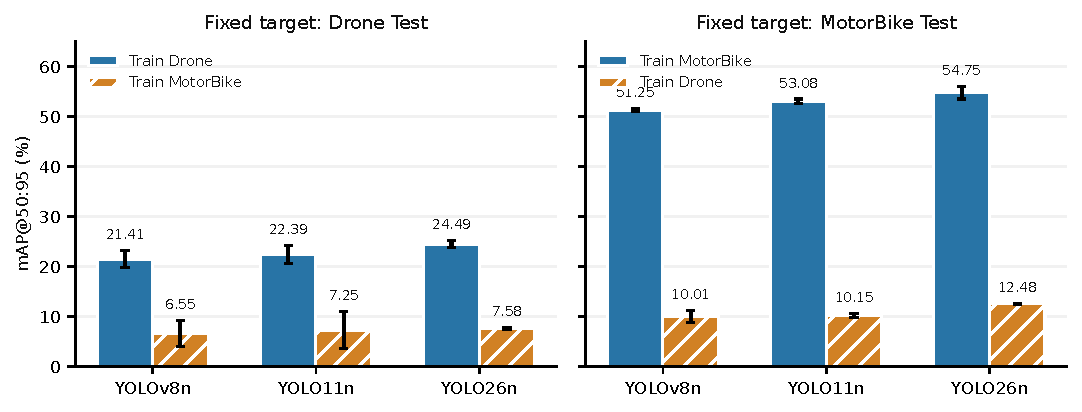
\includegraphics[width=\textwidth]{figures/fixed_target_comparison_light.pdf}
\caption{Full-test performance on each fixed target. Within a panel, training domains change while evaluation images remain identical. Bars show mean mAP@50:95 and error bars sample SD across seeds 13, 37, and 71. All three YOLO variants are included.}
\label{fig:matrix}
\end{figure*}

Table~\ref{tab:gaps} summarizes the paired seed differences. Drone-target mean gaps range from 14.86 to 16.91~pp, whereas MotorBike-target gaps range from 41.24 to 42.94~pp. The corresponding target-asymmetry differences are 26.38, 27.80, and 25.36~pp for YOLOv8n, YOLO11n, and YOLO26n. This consistently larger MotorBike-target advantage is the main asymmetry finding. It does not establish that either platform intrinsically produces more transferable features, because both training composition and the target population differ between these two comparisons.

\begin{table}[t]
\caption{Fixed-target mAP@50:95 advantage (pp, mean $\pm$ sample SD). $H$ is the difference between the two mean gaps.}
\label{tab:gaps}\centering\small
\setlength{\tabcolsep}{4pt}
\begin{tabular}{lrrr}\toprule
Model & Drone Test & MotorBike Test & $H$\\\midrule
YOLOv8n & $14.86\pm1.25$ & $41.24\pm1.04$ & 26.38 \\
YOLO11n & $15.13\pm3.85$ & $42.94\pm0.52$ & 27.80 \\
YOLO26n & $16.91\pm0.80$ & $42.27\pm1.28$ & 25.36 \\
\bottomrule

\end{tabular}
\end{table}

\subsection{RQ2: Seed Consistency and Training Dynamics}
All 18 model--target--seed fixed-target comparisons have positive gaps. The smallest is 10.84~pp for YOLO11n on Drone Test with seed 37. For YOLO26n, Drone-target gaps are 16.91, 16.10, and 17.71~pp for seeds 13, 37, and 71; MotorBike-target gaps are 43.14, 42.87, and 40.80~pp. Thus, the positive direction is not driven by one seed. The supplemental material provides every seed-specific gap.

Variability depends on the particular model and target. For example, the Drone-target gap SD is 3.85~pp for YOLO11n and 0.80~pp for YOLO26n. These three-seed summaries do not establish a general relationship between model generation and optimization stability. The source-validation trajectories in the supplement show that all runs completed 150 epochs, with maximum logged validation mAP occurring between epochs 63 and 133. A validation maximum before the final epoch neither proves global convergence nor establishes that a different schedule would fail to improve performance. The maximum logged mAP is also distinct from independently verifying the fitness rule that saved a checkpoint.

\subsection{RQ3: Class-Level Heterogeneity}
Fig.~\ref{fig:classes} shows per-class differences using the same fixed-target definition. D00, D10, and D20 have positive mean gaps on both targets for all three variants. On MotorBike Test, the D20 advantages are 53.21, 57.72, and 56.45~pp for YOLOv8n, YOLO11n, and YOLO26n, respectively. The corresponding cross-domain D20 AP values are only 2.14\%, 1.00\%, and 1.54\%, compared with in-domain values of 55.35\%, 58.72\%, and 57.99\%. This class is particularly weak under Drone-trained deployment on MotorBike Test.

\begin{figure*}[t]
\centering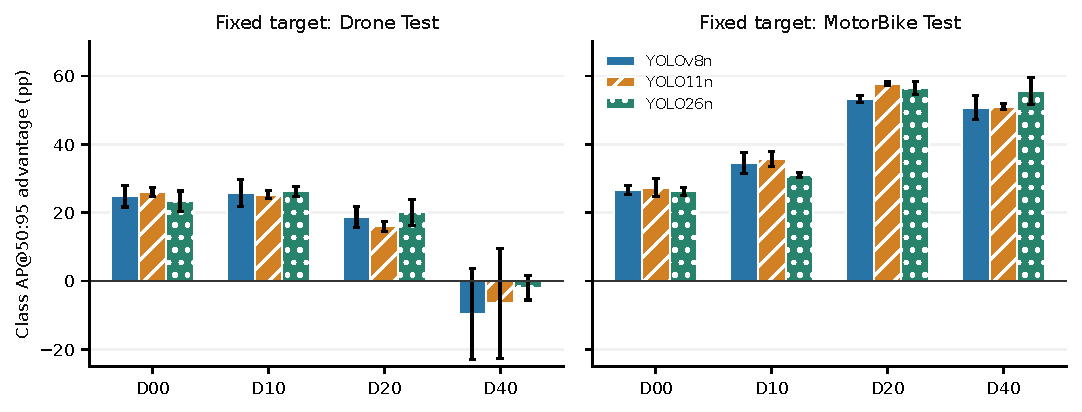
\includegraphics[width=\textwidth]{figures/class_gaps_light.pdf}
\caption{Per-class fixed-target AP@50:95 advantage of target-domain training over training on the other domain. Bars show means and error bars sample SD of seed-specific differences. Negative D40 gaps on Drone Test are retained. Different class supports and scene clustering limit interpretation of these differences.}
\label{fig:classes}
\end{figure*}

D40 behaves differently on Drone Test. Its mean class gaps are $-9.74$, $-6.61$, and $-1.95$~pp for YOLOv8n, YOLO11n, and YOLO26n: MotorBike-trained models have higher mean AP for this class despite the opposite aggregate-mAP result. The recorded Drone test support is only 17 D40 boxes, making class-level interpretation fragile. We retain the class in the primary four-class metric and do not modify the split or labels to remove this result. Complete class AP values are supplied in the supplement. The aggregate mAP does not imply uniform superiority across classes, and the archives do not establish a visual mechanism for any individual failure.

\subsection{RQ4: Accuracy Improvements and Transfer Gaps}
YOLO26n achieves the highest mean in-domain mAP@50:95: 24.49\% on Drone and 54.75\% on MotorBike. Relative to YOLOv8n, the absolute improvements are 3.08 and 3.50~pp, or 14.38\% and 6.83\% relative improvements. The corresponding fixed-target gaps remain 16.91 and 42.27~pp. Under Eq.~\eqref{eq:relative}, these represent relative declines of 69.04\% and 77.20\% against the respective target-trained baselines.

The newer variant therefore improves in-domain mean accuracy without eliminating the cross-domain gap. The gap is not monotonically related to model generation: YOLO26n has a larger Drone-target gap than YOLO11n, but a slightly smaller MotorBike-target gap (42.27 versus 42.94~pp). Nor is it best on every class: YOLO11n has higher in-domain D20 AP on MotorBike Test than YOLO26n (58.72\% versus 57.99\%). These observations support model- and class-specific assessment rather than a universal robustness ranking.

\subsection{Sensitivity to Excluded-Class Images}
All 18 fixed-target comparisons remain positive on the clean-only subsets. Mean Drone-target gaps for YOLOv8n, YOLO11n, and YOLO26n are 15.25, 14.93, and 16.59~pp; the respective MotorBike-target gaps are 41.87, 43.86, and 42.60~pp. The main direction and larger MotorBike-target advantage therefore persist under this restriction. This is a sensitivity check on a changed evaluation population, not evidence that removing excluded labels alone causes the score change. Supplementary tables report the full clean-only matrix and the complementary mAP@50 results.

\section{Discussion}
\subsection{What the Fixed-Target Design Establishes}
The central finding is a substantial domain-associated source-training gap on both targets, replicated across the three tested YOLO variants and seed values. Holding target images fixed removes the ambiguity of comparing scores from different test populations within each gap. It does not equalize the source collections: Drone training contains 1,680 images versus 1,383 MotorBike images, and the collections can differ in geography, road surfaces, illumination, class frequency, and annotation density.

Acquisition-related scale and context changes are plausible contributors, but the experiment does not measure their individual effects. In particular, the larger MotorBike-target gap is not sufficient evidence that MotorBike images provide richer features or that drone altitude is the cause of transfer failure. Paired captures of identical road sections, source-size-matched controls, and direct measurements of object-scale distributions would be needed to examine those explanations.

\subsection{Implications for Deployment}
The results favor validating a detector on the intended acquisition platform before using an in-domain score to guide deployment. Selecting the variant with the highest in-domain mean is insufficient to guarantee small transfer gaps. Operational evaluation should also inspect class-level behavior: a strong aggregate result can coexist with weak D20 transfer or an apparent D40 reversal on a sparsely represented target. A decrease in mAP should not be interpreted as an equal proportional decrease in recall or as a measured maintenance-cost increase; neither follows directly from this metric.

The next practical interventions are target-domain fine-tuning, mixed-domain training, or domain-adaptation strategies evaluated under a newly specified protocol. These interventions were not tested here. Their expected benefit should not be inferred from the present descriptive comparisons.

\subsection{Limitations and Threats to Validity}
\emph{Construct validity:} the scene-review procedure addresses identified similarity links, but undiscovered overlap can remain. Original audit artifacts were not independently replayed during reanalysis, and pre-finalization exposure to some MotorBike images limits an entirely untouched-holdout claim. Excluded annotations are not ignore regions, while clean-only restriction changes image composition.

\emph{Internal validity:} unequal source sizes and correlated acquisition conditions prevent causal attribution to viewpoint. Model-specific architecture, pretraining, loss implementation, and evaluation behavior are not isolated by matching the explicit fine-tuning settings. The comparison does not measure latency, energy, parameter counts, or equal-compute performance.

\emph{Conclusion validity:} the three seed values quantify training variation on fixed datasets. They are not independent scene samples, and the three variants belong to the same YOLO family. No formal significance test, scene-bootstrap interval, or independent inference replay is reported. Agreement between archived CSV and JSON summaries confirms internal consistency of those records, not their correctness against every original image and annotation.

\emph{External validity:} both collections are China subsets of RDD2022. Transfer to another country, acquisition device, annotation policy, or live video stream remains unmeasured. Additional regions require a separate ontology and split audit. These limits make the study a descriptive benchmark analysis rather than a universal or certified leakage-free robustness result.

\section{Conclusion}
Using 18 fine-tuning runs across YOLOv8n, YOLO11n, and YOLO26n, this study finds positive fixed-target in-domain advantages in every model--target--seed comparison on the scene-reviewed RDD2022 Drone/MotorBike partition. Mean gaps are 14.86--16.91~pp on Drone Test and 41.24--42.94~pp on MotorBike Test, with the same direction on the clean-only subsets. Class-level analysis reveals large D20 gaps on MotorBike and negative mean D40 gaps on the sparsely supported Drone target. YOLO26n improves mean in-domain mAP on both domains but does not remove the cross-domain deficit.

The evidence supports explicit target-platform evaluation and class-level reporting. Future work should independently replay per-image predictions, quantify scene-level uncertainty, match source training sizes, and test adaptation or mixed-domain training. Paired-view data would be required to separate acquisition geometry from other collection differences.

\section*{Data Availability and AI Assistance}
RDD2022 is the source dataset\cite{arya2024rdd2022}. The accompanying reproducibility package contains the 72 archived full/clean-only metric rows, run identities, training-log CSVs, summary tables, and scripts that regenerate the light-background figures. Its split identifier is given in Section~III. Original imagery and model weights are not redistributed in this manuscript package. The supplementary document provides class AP, seed-specific gaps, mAP@50, clean-only results, and source-validation curves. Scene-review triage and manuscript preparation used AI assistance; final scene decisions and scientific interpretation remain the authors' responsibility.

\balance
\bibliographystyle{ieeetr}
\bibliography{references}
\end{document}
